\section{Fragen zur Vorlesung}
\begin{enumerate}[a)]
	\item Was ist der Vorteil eines B-Baums gegenüber binären Suchbäumen?

	\begin{solution}
	Größerer Fan-Out (Verzweigungsgrad) $\rightarrow$ Grundidee: Blockzugriff ist teuer, also weniger davon machen.

	Das ist auch der Grund, warum ein Knoten gerade so groß wie ein Block ist. Ein Knoten ist die Einheit, in der wir nach der nächsten Verzweigung suchen. Sie sollte komplett zur Verfügung stehen und keine zwischenzeitlichen I/Os verursachen.
	\end{solution}


	\item Was sind die charakteristischen Eigenschaften eines B-Baums?

	\begin{solution}
	Perfekt balanciert (alle Pfade von der Wurzel zu einem Blatt sind gleich lang), jeder innere Knoten hat zwischen $k+1$ und $2k+1$ Nachfolger. Jeder Knoten außer der Wurzel ist mindestens zur Hälfte gefüllt. Die Wurzel ist ein Blatt (dann besteht der Baum nur aus der Wurzel) oder sie hat mindestens 2 Nachfolger.
	\end{solution}


	\item Was unterscheidet den B*-Baum vom B-Baum? Was sind die Vor- und Nachteile?

	\begin{solution}
	Beim B*-Baum werden die Nutzdaten (Satzadresse, oder auch ganzer Satz bei Primärorganisation) nur in den Blättern gespeichert. Das reduziert die Höhe des Baums (durch den höheren Verzweigungsgrad oben) und erlaubt Bereichsanfragen durch Verkettung der Blätter.
	\end{solution}

	\item Zeichnen Sie schematisch den Aufbau eines Blattknotens und eines inneren Knotens eines B*-Baums.

	\begin{solution}

	Innerer Knoten:

		\begin{center}
		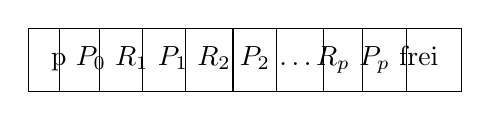
\begin{tikzpicture}

				\node at (2.35, 2.4) {p  $P_{0}$  $R_{1}$  $P_{1}$  $R_{2}$  $P_{2}$  \dots  $R_{p}$  $P_{p}$  frei};

				%Male ausgefülltes Rechteck
				%\fill[fill=lightgray](2.75, 2) rectangle+(0.4, 0.8);

				%Rechteck
				%     links hoehe         rechts hoehe
				\draw (-0.4,2) rectangle +(5.5, 0.8);

				%Senkrechte Striche
				\draw (0, 2) -- (0, 2.8)
							(0.5, 2) -- (0.5, 2.8)
							(1.05, 2) -- (1.05, 2.8)
							(1.6, 2) -- (1.6, 2.8)
							(2.2, 2) -- (2.2, 2.8)
							(2.75, 2) -- (2.75, 2.8)
							(3.35, 2) -- (3.35, 2.8)
							(3.85, 2) -- (3.85, 2.8)
							(4.4, 2) -- (4.4, 2.8)
							;

		\end{tikzpicture}
		\end{center}



	Wobei $P_{i}$ ein Zeiger auf einen weiteren inneren oder Blattknoten und $R_{i}$ ein Referenzschlüssel ist. p ist die Anzahl der Einträge. Es gilt: $k \leq p \leq 2 k$

	Blattknoten:

		\begin{center}
		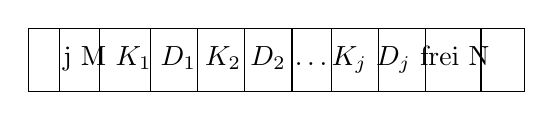
\begin{tikzpicture}

				\node at (2.35, 2.4) {j  M  $K_{1}$  $D_{1}$  $K_{2}$  $D_{2}$  \dots  $K_{j}$  $D_{j}$  frei   N};

				%Rechteck
				%     links hoehe         rechts hoehe
				\draw (-0.8,2) rectangle +(6.3, 0.8);

				%Senkrechte Striche
				\draw (-0.4, 2) -- (-0.4, 2.8)
							(0.1, 2) -- (0.1, 2.8)
							(0.75, 2) -- (0.75, 2.8)
							(1.35, 2) -- (1.35, 2.8)
							(1.95, 2) -- (1.95, 2.8)
							(2.55, 2) -- (2.55, 2.8)
							(3.05, 2) -- (3.05, 2.8)
							(3.65, 2) -- (3.65, 2.8)
							(4.25, 2) -- (4.25, 2.8)
							(4.95, 2) -- (4.95, 2.8)
							;

		\end{tikzpicture}
		\end{center}
	Wobei $K_{i}$ ein Referenzschlüssel ist und $D_{i}$ die Nutzdaten zum Schlüssel $K_{i}$. j ist die Anzahl der Einträge. Es gilt: $k^* \leq j \leq 2 k^*$. $M$ ist der Zeiger auf den vorherigen und $N$ der Zeiger auf den nächsten Blattknoten.

	\end{solution}

	\item Ist in einem B*-Baum jeder Schlüsselwert, der in einem inneren Knoten gespeichert ist, auch in einem Blattknoten vorhanden?

	\begin{solution}
		Nein. Es kann zum Beispiel durch Löschen eines Eintrags in einem Blattknoten die Situation entstehen,
		dass in einem inneren Knoten ein Referenzschlüssel vorkommt, der in keinem Blattknoten mehr enthalten ist. \\
		Selbstverständlich bleibt jedoch die Semantik erhalten, dass vor einem Referenzschlüssel nur Einträge mit niedrigeren
		oder gleichen Schlüsselwerten und nach dem Referenzschlüssel nur Einträge mit höheren Schlüsselwerten vorkommen.
	\end{solution}

	\item Welche Möglichkeiten fallen Ihnen ein, um Einträge wieder aus einem Index zu entfernen?

	\begin{solution}
		Die Einträge können direkt aus dem Index gelöscht werden. Das erfordert jedoch je nach Index und verwendeter Implementierung eine z.\,T. sehr aufwendige Reorganisation. Löschen in Hashtabellen mit quadratischem Sondieren ist komplex bis unmöglich, ohne kompletten Neuaufbau des Indexes. Löschen aus einem B-Baum kann eine ganze Reihe von Unterläufen und im Laufe der Unterlaufbehandlung wieder Überläufen erzeugen.

		Eine andere Möglichkeit ist, die Einträge als "`gelöscht"' zu markieren, ohne sie tatsächlich zu entfernen. So macht es z.\,B. auch Oracle in seinen B-Baum-Indizes. Hierdurch geht das Löschen sehr schnell. Der Speicherbedarf ist durch die gelöschten Elemente aber höher und kann je nach Struktur auch die Kosten für Einfügen und Suchen erhöhen. Der zusätzliche Aufwand hierfür ist abhängig von der Indeximplementierung und der Zahl der Löschvorgänge.

		Als Kompromisslösung bietet es sich an, Einträge als gelöscht zu markieren und ab einem gewissen Punkt, zum Beispiel einem bestimmten Prozentsatz von Platzhaltern in Bezug zur Gesamtzahl an Einträgen, die Tabelle neu aufzubauen. Bei Oracle stehen Informationen über den Zustand des Indexes bereit und der Administrator entscheidet darüber, wann ein Index neu aufgebaut werden soll.
	\end{solution}

	\item Welche Daten müssen und welche können in einem Index gespeichert werden?

	\begin{solution}
		Der Indexwert (Schlüssel) muss immer gespeichert werden. Was zusätzlich noch gespeichert wird, hängt davon ab, für was der Index benutzt werden soll:

		\begin{description}
			\item[Keine weiteren Informationen] Bereits nichts weiter als nur den Indexwert zu speichern kann Anfragen unterstützen, wenn oft überprüft werden soll, ob ein Schlüsselwert vorhanden ist, aber der zugehörige Satz nicht weiter interessiert (z.\,B. für Unique-Attribute oder zur Unterstützung einer \texttt{contains}-Funktion).
			\item[TID] Zusätzlich wird die Satzadresse des Satzes gespeichert. Dadurch wird der Schlüsselzugriff auf den Satz ermöglicht.
			\item[(TID +) Teil eines Satzes] Zusätzlich zum Schlüsselwert und der Satzadresse werden noch ein oder mehrere Felder gespeichert. Das erfordert natürlich einen höheren Platzbedarf, kann aber sinnvoll sein, wenn häufig Anfragen
			gestellt werden, die den Schlüssel und bestimmte Felder benutzen. Man spart sich den Zugriff über die Satzadresse, wenn die benötigten Felder bereits im Index stehen.
			Durch das Weglassen der TID erhält man eine Datenstruktur, die nur bei Anfragen auf die in der Struktur abgelegten Teile verwendet werden kann. Andernfalls ist der Index für diese Anfrage nicht benutzbar.
			\item[Ganzer Satz] Der ganze Satz wird im Index gespeichert. (Primärorganisation)
			\item[Mehrere TIDs, Teile von Sätzen, Sätze] Bei einem Index über ein nicht-eindeutiges Attribut kann es zu einem Schlüsselwert mehrere Tupel geben. Diese werden dann alle zusätzlich zum Schlüsselwert abgelegt. Hierfür sind, genauso wie für die Ablage variabel langer Sätze in einem Index, angepasste Index-Algorithmen notwendig, die variabel lange Einträge unterstützen.
			\item[TIDs, Teile von Sätzen, Sätze anderer Relationen] Bei einem Index über einen Primärschlüssel können sowohl die TIDs der beinhaltenden Relation als auch die TID der referenzierenden Relation mit Fremdschlüssel gespeichert werden, um den Join zu erleichtern. Natürlich lassen sich bei dieser Vorgehensweise alle anderen Optionen (Teile des Satzes, Ganzer Satz) genauso anwenden.
		\end{description}

		%Indexwert muss, TID, ganzes Tupel, Teil eines Tupels kann. Nur Indexwert könnte auch sinnvoll sein, wenn nur auf Vorhandensein geprüft werden soll.
	\end{solution}
\end{enumerate}

\begin{note}
Darauf hinweisen, dass B-Bäume der Standard bei der Implementierung von Indizes sind.

Außerdem darauf hinweisen, dass die Bezeichnung B$^\text{+}$-Baum dasselbe Konzept
meint, das wir als B*-Baum bezeichnen.
\end{note}


